\documentclass{frontiersSCNS} % for Science articles

\usepackage{url,lineno}
\usepackage{color}
\usepackage{enumerate}
\linenumbers
\usepackage{bbm}
\usepackage{centernot}

%%  Our commands
\DeclareMathOperator{\Tr}{tr}
\newcommand{\mcond}{\,\middle\vert\,}
\newcommand{\cond}{\,\vert\,}
\newcommand{\T}{\intercal}
\newcommand{\TODO}[1]{\emph{\tiny\color{Rhodamine}$\langle\langle$#1$\rangle\rangle$}}
\newcommand*\dif{\mathop{}\,d}

% Leave a blank line between paragraphs instead of using \\

\copyrightyear{}
\pubyear{}

\def\journal{Computational Neuroscience}
\def\DOI{}
\def\articleType{Research Article}
\def\keyFont{\fontsize{8}{11}\helveticabold }
\def\firstAuthorLast{Yatsenko {et~al.}} %use et al only if is more than 1 author
\def\Authors{
Dimitri Yatsenko\,$^{1,*}$, 
Alexander Ecker\,$^{2,1}$,
Emmanouil Foudarakis\,$^{1}$,
R.~James Cotton\,$^{1}$,
Kre\v{s}imir Josi\'{c}\,$^{3}$,
and Andreas S.~Tolias\,$^1$}

% Affiliations should be keyed to the author's name with superscript numbers and be listed as follows: Laboratory, Institute, Department, Organization, City, State abbreviation (USA, Canada, Australia), and Country (without detailed address information such as city zip codes or street names).
% If one of the authors has a change of address, list the new address below the correspondence details using a superscript symbol and use the same symbol to indicate the author in the author list.
\def\Address{
$^{1}$Department of Neuroscience, Baylor College of Medicine, Houston, TX, USA\\
$^{2}$Max Planck Institute of Biological Cybernetics, T\"ubingen, Germany\\
$^{3}$Department of Mathematics and Department of Biology and Biochemistry, University of Houston, Houston, TX, USA
}
% The Corresponding Author should be marked with an asterisk
% Provide the exact contact address (this time including street name and city zip code) and email of the corresponding author
\def\corrAuthor{Dimitri Yatsenko}
\def\corrAddress{Andreas Tolias Lab, Department of Neuroscience, Baylor College of Medicine, One Baylor Plaza, Houston, TX 77030, USA}
\def\corrEmail{yatsenko@cns.bcm.edu}

% \color{FrontiersColor} Is the color used in the Journal name, in the title, and the names of the sections

\begin{document}
\onecolumn
\firstpage{1}

\title[Improved estimates of neural correlations]{Improved estimates of neural correlations suggest detailed interactions in visual cortex}
\author[\firstAuthorLast ]{\Authors}
\address{}
\correspondance{}
\editor{}
\topic{Research Topic}

\maketitle
\begin{abstract}
Correlations between the spiking activity of pairs of neurons are among the most familiar descriptive statistics of neural activity. Multineuronal recordings provide richer information than the equivalent number of neuron pairs. For example, the full covariance matrix reveals correlated activity across the entire population as well as partial correlations between pairs.  Estimation of covariance matrices can be improved by regularization, \emph{i.e.}\;by imposing some kind of structure.  Optimal regularization must be determined empirically since its effect depends on how closely the imposed structure matches the underlying regularities. For example, we can use low-rank parameterizations of the covariance matrix to account for common fluctuations across the recorded population. Conversely, if correlations are strongly influenced by a small fraction of pairwise linear associations between the observed neurons, we can impose sparsity on the inverse covariance matrix. We can also use a `sparse+low rank’ inverse covariance representation to account for both common fluctuations and pairwise interactions.  

To select the optimal structure of neural correlations in a local neural circuit, we compared the performance of several covariance estimators on the activity of 100--300 neurons in mouse visual cortex: sample covariance, covariance shrinkage, factor analysis, sparse inverse covariance, and sparse+low-rank inverse covariance. We inferred instantaneous firing rates in 200 ms bins from the somatic calcium signals acquired with fast 3D random-access two-photon microscopy.  Each covariance estimator was optimized and evaluated by cross-validation. As expected, covariance shrinkage reliably outperformed the sample covariance estimate. In turn, factor analysis-based estimates significantly outperformed covariance shrinkage. Yet sparse inverse covariance with or without an additional low-rank component significantly outperformed both factor analysis and shrinkage estimators. The superior performance of the sparse inverse covariance estimator suggests the relative importance of detailed network interactions over common diffuse input in the circuit we studied.


%As a primary goal, the abstract should render the general significance and conceptual advance of the work clearly accessible to a broad readership. References should not be cited in the abstract.
%See the Summary Table at \\ \url{http://www.frontiersin.org/}\texttt{\jour nal}\url{/authorguidelines} \\for abstract requirement and length according to article type.


\tiny
 \keyFont{ \section{Keywords:} population activity, neural circuits, functional connectivity, neural correlations, noise correlations, regularization, covariance estimation} %All article types: you may provide up to 8 keywords; at least 5 are mandatory.
\end{abstract}


\section{Introduction}
% For Original Research Articles, Clinical Trial Articles, and Technology Reports the introduction should be succinct, with no subheadings.
%
%For Clinical Case Studies the Introduction should include symptoms at presentation, physical exams and lab results.
%
\hl{\tiny why correlations:}
Linear correlations between the spiking activity of pairs of neurons, or simply \emph{neural correlations}, are among the most familiar descriptive statistics of neural population activity \citep{Cohen:2011}.   
For example, \emph{noise correlations}, i.e.~the correlations of stimulus response variability between pairs of neurons in sensory areas, have been of particular interest thanks, in part, to their profound theoretical implications for stimulus coding \citep{Zohary:1994,Abbott:1999,Averbeck:2006,Berens:2011}.
Lending further credence to their role as indicators of detailed and specific functional organization have been a series of discoveries of nontrivial relationships between neural correlations and other aspects of circuit organization such as the physical distance separating the neurons, their synaptic connectivity and stimulus tuning similarity, cortical layer specificity, cell-type specificity, progressive changes in development and in learning, changes due to sensory stimulation and global brain states, and others \citep{Kohn:2005,Smith:2008,Kohn:2009,Goard:2009,Golshani:2009,Renart:2010,Ecker:2010,Smith:2013,Denman:2013}. 

\hl{\tiny ambiguity of interpretation:}
Neural correlations do not come with ready or unambiguous mechanistic interpretations.   
Theoretical and simulation studies show that neural correlations at various temporal scales may arise from any combination of underlying mechanisms such as direct synaptic interactions,  common or correlated inputs, shared sensory noise, chains of multiple synaptic connections, oscillations, top-down modulation, and background network activity \citep{Perkel:1967b,Shadlen:1998,Salinas:2001,Ostojic:2009,Rosenbaum:2011}

\hl{\tiny opportunities with multineuronal data:}
Early studies of neural correlations were based on measurements from isolated pairs of neurons and their impact on coding was extrapolated to entire populations \citep{Shadlen:1998,Zohary:1994}.  Modern massively multineuronal recordings allow estimations of entire correlation matrices from large neuronal populations, which provide more information than the equivalent number of pairwise correlations assessed in isolation.
After all, the correlation matrix is greater than the sum of its parts: it can be transformed into other representations  that accentuate different aspects of its structure and may suggest different mechanistic interpretations.  
For example, the eigenvalue decomposition, also known as the principal component analysis, of the covariance matrix expresses shared correlated activity components across the entire population;  common fluctuations of population activity of the entire circuit may be accurately represented by just a few principal components but will affect all correlation coefficients. 
In contrast, the off-diagonal elements of the inverse of the correlation matrix constitute scaled partial correlations between neuron pairs, which reflect their specific linear dependencies, after accounting for all other recorded cells;
a strong interaction between a pair of neurons may be expressly represented by a single partial correlation but its effects propagate to multiple correlations and principal components.

\hl{\tiny motivate regularization} Estimation of parameters of the covariance matrix from data is inherently challenging, increasingly for very high-dimensional data. As the amount of data grows only linearly with population size, the number of free parameters in a complete representation of the covariance matrix increases quadratically, multiplying opportunities for spurious patterns to emerge among the correlations. 
Although the estimation error of each covariance coefficient, in isolation, is unaffected by the dimensionality of the data, the estimation error of other parameters of the covariance matrix increases with population size.  
For example, the large eigenvalues of in the sample covariance matrix are biased upward while small eigenvalues are biased downward, with both variance and bias increasingly large with increasing data dimensionality \citep{Hayes:1981}.  Similarly, the coefficients of the inverse covariance matrix require  larger sample sizes to be estimated accurately in high-dimensional data.

\hl{\tiny forms of regularization} The convergence of the estimate of multivariate parameters to their true values can be improved through \emph{regularization},  Regularization is the deliberate biasing or \emph{shrinkage} of the empirical estimate toward a less variable \emph{target estimate} \citep{Schafer:2005} or the deliberate restriction of the estimate to a lower-dimensional space \citep{Dempster:1972,Fan:2008,Friedman:2008,Rothman:2008}. 
\hl{\tiny The two definitions overlap and are often equivalent, but not always, according to James, but I would like to see an example of shrinkage that is not, effectively, a low dimensional parameterization of the original problem.} 
One intuitive explanation of regularization is as the addition of some  prior knowledge about the likely forms of the covariance matrix. Curiously, though, regularization need not reflect any accurate knowledge about the nature of covariance matrices in general or in the particular domain. Some improvement arises due to \emph{Stein's phenomenon}, i.e. the favorable tradeoff between bias and variability \emph{anytime} a moderate bias toward a less variable target is introduced.  
However, the incorporation into the regularization scheme of real knowledge about the probable forms of covariance matrices for a specific situation will likely confer additional advantage and improve the convergence more substantially than an \emph{ad hoc} regularizer.

%Estimator improvements due to regularization depend profoundly on the parameterization to which it is applied.  Sparsification of the eigenspectrum produces a low-rank estimate of the covariance matrix also known as truncated PCA \citep{Rothman:2008} or, allowing for additional independent variances, as factor analysis (FA) \citep{Fan:2008}.  Sparsification of the inverse covariance is known as covariance selection \citep{Dempster:1972,Friedman:2008} and is related to finding a graphical model in which a large fraction of neuron pairs are conditionally independent of each other.  Representations that are capable of concentrating the significant real effects in a small number of parameters will reap greatest benefits from sparsification over ones that distribute the real effects widelyacross many parameters.  Random noise tends to be broadly distributed across all parameters in any parameterization. 

Two questions must be answered in the choice of the regularization scheme: what kind of regularization and how much regularization. The answer to the first question is domain-specific and is often motivated by theories of the origins of correlations in the specific subject domain.  


\hl{\tiny approach and summary of findings} 
In this study, we compared the performance of several covariance estimation schemes for spatially compact groups of 150--300 neurons in layers 2-4 in mouse primary visual cortex during visual stimulation.   The performance of the estimators was evaluted by computing the mean squared error between the optimized covariance estimate fitted to training data and the non-regularized covariance matrix from a separate test data set.  Low-rank covariance estimates performed significantly better than shrinkage estimators, but estimators with sparse partial correlations were more efficient still. Typically, between 3 and 16\% of neuronal paris were connected by non-zero partial interactions.  Mixed sparse estimators with sparse partial correlations and low-rank components performed comparably. 

As noted above, the optimal covariance estimator is domain-dependent. 
These specific findings may not spread to all neural circuits.
Improved accuracy estimation accuracy is not the main aim or the only benefit.  
The selection of the optimal regularization scheme in itself serves as an effective descriptor of the dominant correlation structures. The finding that a identifiable subsets of partial correlations were important to describe the partial correlation makes such pairs as prime candidates as direct functional interactions. 


%\begin{methods}

\section{Material \& Methods}
\subsection{Data acquisition}
Describe the two-photon experiment, refer to Fig.\;1.

\begin{figure}
\centering
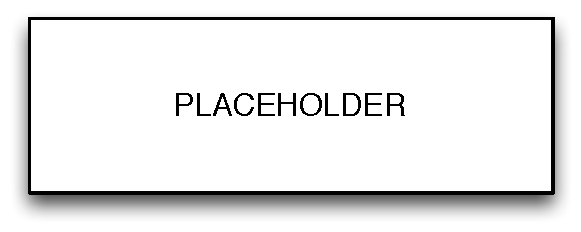
\includegraphics[width=0.5\textwidth]{figures/placeholder.pdf}
\caption{
%\textbf{Figure 1.}{
Experimental setup and data acquisition. 
\textbf{A}: Mouse in two-photon microscope, visual stimulation, 3D scanning of cells.
\textbf{B}: Calcium signals
\textbf{C}: Deconvolution and binning.
}\label{fig:01}
%}
\end{figure}




\section{Theory of covariance estimation}
\subsection*{The sample covariance matrix}
We aim to estimate the true covariance matrix $\Sigma = \E{(x-\mu)(x-\mu)^\T}$ of the instantaneous activity vector $x$ of a population of $p$ neurons. Here $\E{\cdot}$ denotes expectation \TODO{for the true data generating process} and $x$ is the $p\times 1$ vector of real-valued instantaneous firing rates discretized into bins of duration $\Delta t$ and $\mu = \E{x}$.  

For detailed explanation of the notation, definitions, and derivations, see Appendix. 

The usual estimator of $\Sigma$ is the sample covariance matrix
\begin{equation}
\hat \Sigma_0 = \frac 1 \nu \sum\limits_{t=1}^n (x(t)-\mu)(x(t)-\mu)^\T 
\end{equation}
where $x(t),\;t=1,\ldots,n$ are sequential observations of population activity inferred from calcium signals; $\nu$ is the number of degrees of freedom. For independent observations $\nu=n-1$ because estimation of the mean $\mu$ accounts for one degree of freedom. When observations are correlated, as is the case with calcium signals, $\nu < n-1$ and may be estimated from the signal. 

The sample covariance matrix is constructed to be unbiased, so that $\E{\hat\Sigma_0} = \Sigma$. 

\subsection*{Evaluation of covariance matrix estimators}
The quality of a covariance matrix estimate $\hat\Sigma$ is measured by a real-valued \emph{loss function} $\loss{\hat\Sigma,\Sigma}$.  The loss function quantifies the deviation of $\hat\Sigma$ from $\Sigma$ and attains its minimum  when $\hat\Sigma = \Sigma$.  \Kcomment{Could we say that it quantifies the error in the estimate?}

For the purposes of this study, we adopted the \emph{negative normal log-likelihood loss} function:
\begin{equation}\label{eq:loss}
\loss{\hat\Sigma,\Sigma} = \frac 1 p\left[\ln \det \hat \Sigma + \Tr(\hat \Sigma^{-1}\Sigma)\right]
\end{equation}
This choice is motivated by mathematical convenience. Other popular choices for the loss function are the Frobenius norm of the difference $\hat\Sigma-\Sigma$ \cite{Ledoit:2004,Schafer:2005}, Stein's entropy loss, and quadratic loss \cite{James:1961,Fan:2008}.  We expect that the main conclusions of our study will not change qualitatively under other well behaved loss functions.

The aim of our project is to produce covariance matrix estimates that minimize the expected loss 
\begin{equation}
r = \E{\loss{\hat\Sigma, \Sigma}}
\end{equation}
which is known as the \emph{risk} of $\hat\Sigma$.

In practice, the true value $\Sigma$ is not accessible and an estimators' risks must be estimated from the data.  This may be accomplished through \emph{validation}.  \Kcomment{If you will discuss validation later, point to it.}
Let $\hat\Sigma_0^\prime$ denote a sample covariance matrix measured from an independent sample that was not used included in the computation of $\hat\Sigma$. 

$\loss{\cdot,\cdot}$ is additive in its second argument so that \Kcomment{You frequently use ``such that'' instead of ``so that''}
 \begin{equation}\label{eq:additivity}
 \loss{\hat\Sigma,X_1} + \loss{\hat\Sigma,X_2} \equiv \loss{\hat\Sigma,X_1+X_2}
 \end{equation}
Then \emph{validation loss}  \TODO{check appropriate term}
\begin{equation}\label{eq:validationLoss}
\hat \ell = \loss{\hat\Sigma,\hat\Sigma_0^\prime}
\end{equation}
is an unbiased estimate of the risk:
 \begin{equation}\label{eq:empiricalRisk}
\E[(\hat\Sigma, \hat\Sigma_0^\prime)] {\hat\ell} 
= \E[(\hat\Sigma, \hat\Sigma_0^\prime)]{\loss{\hat\Sigma,\hat\Sigma_0^\prime}}
= \E{\loss{\hat\Sigma,\E{\hat\Sigma_0^\prime}}}
= \E{\loss{\hat\Sigma,\Sigma}} = r
 \end{equation}
Therefore, estimators resulting in consistently lower validation loss can be inferred to produce estimates that are closer to truth than estimators with higher validation loss.
\Kcomment{This is probably not a very insightful question -- but why do we assume that the sample covariance
is what we compare $\hat\Sigma$ when we validate the results.  Our point is that this estimate is not very good.}

Other popular loss functions such as entropy loss do not comply with Eq.~\ref{eq:additivity} and their validation loss is not an unbiased estimate of risk.

Since $\loss{\cdot,\cdot}$ is equivalent to negative normal log likelihood, the above derivation has led to the familiar criterion that the optimal covariance matrix estimator is one that consistently maximizes cross-validated normal log likelihood.


\section{Simulation}
\subsection{Simulation}
To illustrate,


\section{Results}
\subsection*{Data acquisition}
We recorded the calcium activity  of dense populations of neurons in the supragranular layers in primary visual cortex of anesthetized mice using fast random-access 3D scanning two-photon microscopy \cite{Stosiek:2003,Reddy:2005}.  Numerious repetitions of full-field drifting gratings (Fig. 1A and 1B) were presented to the eye contralateral to the imaged site. This technique allowed recording from a large number (150--350) of cells in a small volume of cortical tissue ($200\times200\times100$ $\mu$m$^3$) in layers 2/3 and 4. Somatic calcium signals were deconvolved using  sparse nonnegative deconvolution \cite{Vogelstein:2010} (Fig.\;1C and 1D).  The average stimulus response was subtracted to remove stimulus covariance and the sample noise covariance matrix was computed (Fig.\;1E).

\begin{figure}[htp]
\begin{center}
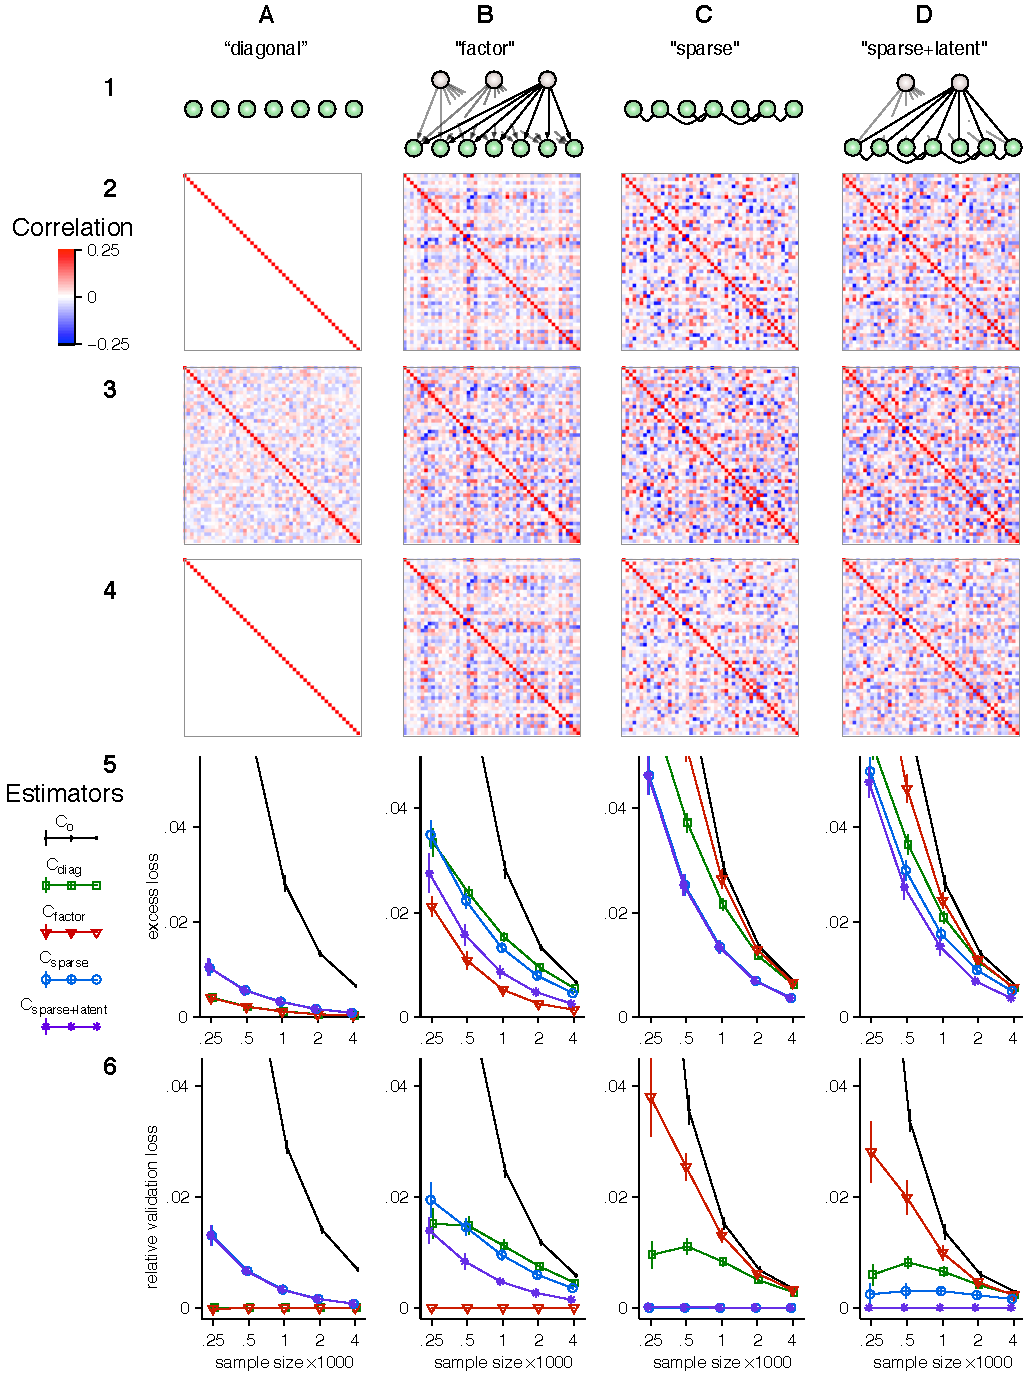
\includegraphics[width=2.5in]{figures/Figure1.pdf}
\end{center}
\caption{
{\bf Acquistion of neural population activity using two-photon fluorescence imaging of calcium signal.}  {\bf A.} Visual stimuli comprising brief (500 ms) presentatios of full-field drifting gratings separated by blank screens. {\bf B.} Two-photon fast 3D imaging of calcium signals in an awake mouse. {\bf C.} Deconvolved calcium signals. {\bf D.} The sample covariance matrix of neuronal calcium signals in 200 ms time bins. 
}
\label{Figure_label}
\end{figure}


\subsection*{The sample covariance matrix}
We aim to estimate the true covariance matrix $\Sigma = \E{(x-\mu)(x-\mu)^\T}$ of the instantaneous activity vector $x$ of a population of $p$ neurons. Here $\E{\cdot}$ denotes expectation \TODO{for the true data generating process} and $x$ is the $p\times 1$ vector of real-valued instantaneous firing rates discretized into bins of duration $\Delta t$ and $\mu = \E{x}$.  

For more rigorous notation, definitions, and derivations, see Appendix. 

The usual estimator of $\Sigma$ is the sample covariance matrix
\begin{equation}
\hat \Sigma_0 = \frac 1 {n-c} \sum\limits_{t=1}^n (x(t)-\mu)(x(t)-\mu)^\T 
\end{equation}
where $x(t),\;t=1,\ldots,n$ are sequential observations of population activity inferred from calcium signals. Bessel's correction $c$ makes the estimate unbiased such that $\E{\hat\Sigma_0} = \Sigma$. When observations $x(t)$ can be assumed to be independent then $c=1$; but when observations are correlated $c>1$ may be estimated from the data. 

\subsection*{Evaluation of covariance matrix estimates}
The quality of a covariance matrix estimate $\hat\Sigma$ is measured by a real-valued \emph{loss function} $\loss{\hat\Sigma,\Sigma}$.  The loss function quantifies the deviation of $\hat\Sigma$ from $\Sigma$ and attains its minimum  when $\hat\Sigma = \Sigma$. 

For the purposes of this study, we adopted the \emph{negative normal log-likelihood loss} function:
\begin{equation}\label{eq:loss}
\loss{\hat\Sigma,\Sigma} = \frac 1 p\left[\ln \det \hat \Sigma + \Tr(\hat \Sigma^{-1}\Sigma)\right]
\end{equation}
This choice is motivated by mathematical convenience. Other popular choices for the loss function are the Frobenius norm of the difference $\hat\Sigma-\Sigma$, Stein's entropy loss, and quadratic loss \cite{James:1961,Ledoit:2004,Schafer:2005,Fan:2008}.  We assert that the main conclusions of our study are unlikely to change drastically other well behaved loss functions.

The aim of our project is produce covariance matrix estimates that minimize the expected loss.  The expected loss of an estimator is known as its \emph{risk}: 
\begin{equation}
r = \E{\loss{\hat\Sigma, \Sigma}}
\end{equation}

In practice, the true value $\Sigma$ is not accessible and estimators' risks must be estimated from the data.  This may be accomplished through validation: 
Let $\hat\Sigma_0^\prime$ denote a sample covariance matrix measured from an independent sample that was not used included in the computation of $\hat\Sigma$. Then \emph{empirical loss} is 
\begin{equation}
\hat \ell = \loss{\hat\Sigma,\hat\Sigma_0^\prime}
\end{equation}
 and its expected value or \emph{empirical risk} is
\begin{equation}\label{eq:empiricalRisk}
\hat r = \E{\hat\ell} = \mathbb E_{\hat\Sigma} \left[ \mathbb E_{\hat\Sigma_0^\prime} \left[ {\loss{\hat\Sigma,\hat\Sigma_0^\prime}} \right] \right]
\end{equation}
Because the chosen loss function is linear in its second argument in the sense that
\begin{equation}
\loss{\hat\Sigma,X_1} + \loss{\hat\Sigma,X_2} \equiv \loss{\hat\Sigma,X_1+X_2}
\end{equation}
the expection on the second argument in Eq.~\ref{eq:empiricalRisk} may be taken inside the loss function:
\begin{equation}
\hat r = \E{\loss{\hat\Sigma,\E{\hat\Sigma_0^\prime}}}  = \E{\loss{\hat\Sigma,\Sigma}} = r
\end{equation}
Thus the empirical loss $\loss{\hat \Sigma,\hat \Sigma_0^\prime}$ serves as an unbiased estimate of risk $r$. 

Because the loss function is equivalent to the negative normal log likelihood, the above derivation led us to the familiar criterion that the optimal covariance matrix estimator is one that consistently maximizes the normal log likelihood of the validation dataset.

\subsection*{Regularization}
Under many loss functions\footnote{
The strict equality in Eq.~\ref{eq:bias-variance} does not hold under the loss function in Eq.~\ref{eq:loss}. However, the equality does hold for its close cousin, Stein's \emph{entropy loss},  which only differs by the order of its arguments and a constant offset: $\mathcal L_s(\hat\Sigma,\Sigma) \equiv \loss{\Sigma,\hat\Sigma} - \loss{\Sigma,\Sigma}$. This defficiency presents no difficulty because we minimize the risk directly, without assessing the two error components individually. The bias-variance decomposition is presented here to motivate the use of regularization.}, 
the estimator's risk can be decomposed as the sum
\begin{equation}\label{eq:bias-variance}
r = b + \varepsilon
\end{equation}
of \emph{approximation error} (``bias'' or systematic error)
\begin{equation}
b = \loss{\bar\Sigma,\Sigma}
\end{equation}
and \emph{estimation error} (``variance'') 
\begin{equation}
\varepsilon = \E{\loss{\hat\Sigma, \bar\Sigma}}
\end{equation}
where $\bar\Sigma = \E{\hat\Sigma}$ is the expected value of the estimate. 

The unbiased estimator $\hat\Sigma_0$ makes $\bar\Sigma=\Sigma$ and thus minimizes  approximation error, but may be excessively susceptible to sample noise and result in high estimation error.

The estimator risk can be reduced by \emph{regularization}. Regularization is the deliberate biasing (\emph{``shrinkage''}) of the estimate toward a low-dimensional, less variable \emph{target estimate} \cite{Bickel:2006,Ledoit:2004}. A regularized estimator solves the bias-variance tradeoff to produce a biased but less variable estimates aiming to minimize the estimator's risk.  Many popular covariance estimators use single pre-determined target estimator and optimize the shrinkage intensity.  Others emphasize the optimal selection of the low-dimensional target estimate from a family of estimates. Yet others effectively combine shrinkage and selection.

We evaluated four regularized estimators denoted here as A, B, C, and D.  Their target estimates correspond to covariance matrices of Gaussian graphical models depicted in Figure 2.  The green spheres represent the recorded neurons, whereas the light-colored spheres represent latent units of the graphical model and the edges connecting them represent conditional dependencies. 

\begin{figure}[htp]
\centering
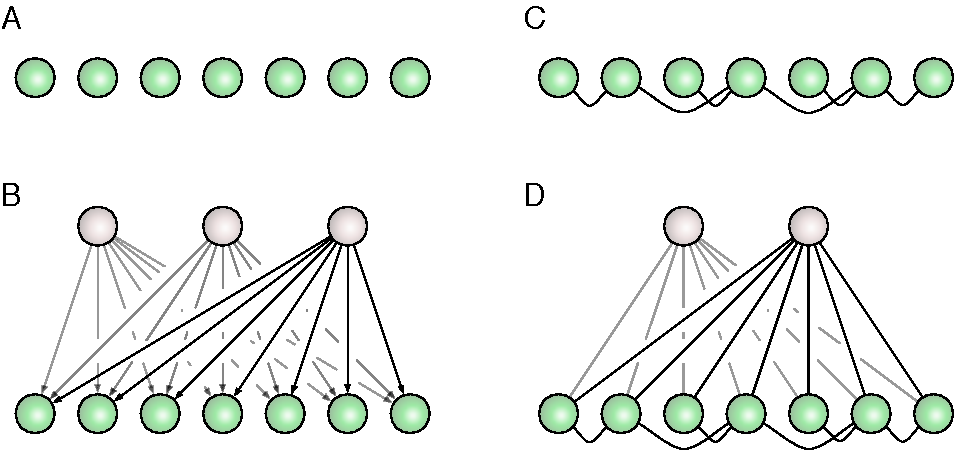
\includegraphics[width=0.5\textwidth]{figures/Figure2.pdf}
\caption{
Graphical models corresponding to the low-dimensional targets of the four regularization schemes used in the paper.
\textbf{A}: A diagonal matrix corresponds to a Gaussian graphical model with no dependencies.
\textbf{B}: In factor analysis, observed nodes are assumed to be influenced by several latent units (``factors") but are otherwise independent.
\textbf{C}: Graphical model with conditional dependencies between a specified subset of pairs of observed neurons, no latent units. 
\textbf{D}: Graphical model with conditional dependencies between a specified subset of pairs of observed neurons and dense interactions with a few latent units.
}\label{fig:02}
\end{figure}


A \emph{graphical model} is a multivarate probability distribution with a specified graph of conditional dependencies between its variables \cite{Koller:2009}.  When this distribution is a multivariate normal distribution, the model becomes a \emph{Gaussian graphical model} or, equivalently, a \emph{Gaussian Markov Random Field}.  Gaussian graphical models have a straightforward relationship to their covariance matrix $\Sigma$:  Zero elements in the inverse of $\Sigma$ indicate conditional independence between the corresponding pair of variables.  

Fitting a graphical model to data involves two tasks: (1) the selection of the set of non-zero covariances or \emph{covariance selection} \cite{Dempster:1972} and (b) the fitting of the non-zero elements.

\emph{Estimate A} is shrinkage estimator toward an independent model.  
\begin{equation}
\hat T_\alpha = (1-\alpha)(\hat\Sigma_0 \circ I) + \frac \alpha p \mbox{tr}(\hat \Sigma_0)I
\end{equation}
where $\circ$ is the entrywise product (Hadamard product). When $\alpha=0$, $\hat T_\alpha$ has the average variance along the diagonal. When $ \alpha=1$, $ \hat T_\alpha$ has empirical variances on the diagonal.

If dependencies between neurons are strictly linear, then a diagonal covariance matrix represents the case where neurons are independent, with no interactions.

The overall estimate $\hat\Sigma$ is found by linear mixing of $\hat\Sigma_0$ and $ \hat T_\alpha$ controlled by the mixing proportion $\lambda$:
\begin{equation}
\hat\Sigma = (1-\lambda)\hat\Sigma_0 + \lambda\hat T_\alpha 
\end{equation}

The hyperparameters $ \alpha$ and $ \lambda$ can be optimally selected from the training data by nested cross-validation.

\subsubsection*{Estimate B: Shrinkage toward }
In estimator B, the target is the multifactor model $ \hat T_d$ with $ d$ latent units. When all dependencies are linear, factor models correspond to mutually independent neurons each influenced by $ d$ latent units. (This is  the conventional factor analysis).

Just as in A, the overall estimate is found by linear mixing:
\begin{equation}
\hat\Sigma = (1-\lambda)\hat\Sigma_0 + \lambda\hat T_d
\end{equation}

\subsubsection*{Estimate C}
In estimate C, the target $ \hat S_\alpha$ is a matrix whose inverse is \emph{sparse}, with a large fraction of off-diagonal elements fixed at zero. The coefficient $ \alpha$ controls the sparsity in $ \hat S_\alpha$.

In models with only linear dependencies, zeros in the inverse covariance indicate conditional independence. Thus the target estimate is depicted as the graphical model with sparse interneuronal interactions.

In practice the target $\hat S_\alpha$ is found by an $ L_1$-norm optimization technique, which combines dimensionality reduction and shrinkage into a single computationally efficient algorithm.

Just as in the previous estimators, the optimal value of the regularization parameter $ \alpha$ is determined from the data by nested cross-validation.

\subsubsection*{Estimate D}
In estimate D, the target $\hat R_{d,\alpha}$ is the matrix whose inverse is the sum of a sparse matrix $\hat S_\alpha$ and a low-rank matrix $\hat L_d$ of rank $d$.
\begin{equation}
\hat R_{d,\alpha} = (\hat S_\alpha + \hat L_d)^{-1}
\end{equation}

If all dependencies are linear, the estimate D describes a group of neurons where each interacts with a small number of latent units and a small fraction of the observed neurons. 

\subsection*{Sparse inverse covariance with a low-rank component dominates other estimators}
I computed noise covariances of population activity from 31 sites.  In each site, I compared the cross-validated performance of the covariance matrix using the Gaussian log-likelihood loss function between the trained estimate $ \hat\Sigma$ and the testing sample covariance $ \Sigma_0^\prime$:
\begin{equation}
\mathcal L(\hat\Sigma,\hat\Sigma_0^\prime) = 
\frac 1 p\left( \ln \det \hat \Sigma + \mbox{tr}(\hat \Sigma^{-1}\hat\Sigma_0^\prime) \right) 
\end{equation}

I obtained the following in figure 3.

This is the full matrix of all comparisons of the estimators.  The plots represents the histograms of the differences of the loss function between the pair of estimators for all 31 sites.  When the differences are positive, the first estimate in the title outperforms the second estimate.

Of particular interest is the first row, which shows that all regularized estimates  outperformed the sample covariance estimate.  Even more informative is the last column, which shows that estimate D (sparse+lowrank) significantly outperformed all other estimates.





\section{Discussion}
\hl{The discussion section is not ready for any feedback. Currently it's just a trashbin with clips from scrapped versions of the introduction. -- Dimitri}

Fundamental questions in systems neuroscience concern the relationship between the function of neural microcircuits and their cytoarchitecture: circuit topology, cell types, and patterns of synaptic connectivity. 

Considerable progress has been made in sensory areas where the functional characterizations of cells are defined by their reproducible responses to external stimuli (reviewed in \citep{Reid:2012}). 

Many key questions in neuroscience revolve around the relationship between the cytoarchitecture of neural microcircuits and the functional organization of their activity \citep{Reid:2012}.  Investigators in this line of inquiry aim to construct networks of functional associations within groups of neurons inferred from observations of their activity under a variety of conditions.  The inferred functional network  could then related to the synaptic connectivity patterns, cell types, cell properties, or the cells' spatial arrangment in the attempt to uncover organizational principles of neural computation. In addition, the network itself can serve as subtrate for subsequent graph-theoretical analysis \citep{Feldt:2011}

Advances in electrophysiology and optical imaging have enabled simultaneous recordings from dozens to hundreds or thousands of cells. 
In particular, recent advances in two-photon imaging of calcium signals have allowed in vivo recordings from nearly every neuron brain-wide in zebrafish \citep{Leung:2013,Ahrens:2013} and in a 3D volume of a few hundred microns in diameter in mouse neocortex \citep{Katona:2012,Cotton:2013}.    
Ambitious projects currently under way aim to record the spiking activity of large fractions of cells from entire circuits and systems in behaving animals \citep{Alivisatos:2012}.  Direct observations of the population activity  of entire circuits open new possibilities for incisive statistical descriptions of the functional connectivity in the circuit.  


One general approach is to construct statistical models reflecting hypothesized models of neural circuit function, including temporal dynamics, nonlinear interactions between neurons, and background network activity \citep{Pillow:2008,Buonomano:2009,Yu:2009}. 
Another general approach is to search for alternative statistics that best describe the population activity without assuming a specific model.  Such evaluations rely on constructing surrogate datasets \citep{Okun:2012} or maximum-entropy distributions that reproduce the statistic of interest \citep{Ganmor:2011,Tkacik:2012} with subsequent testing of how well such constructs can reproduce other observed properties of population activity.

Such more sophisticated statistical descriptions are unlikely to entirely replace neural correlations as the initial descriptive statistic of population activity in experimental neuroscience. Neural correlations have several strengths that will ensure their continued prominence: (a) correlations are well established, familiar, and intuitive to most researchers in biological sciences, (b) correlations are easy to estimate as they are less susceptible to the curse of dimensionality than more sophisticated models, (c) correlations make relatively weak mechanistic assumptions (at the cost of not revealing many potentially important aspects), and (d) correlations serve as input into other models of population activity or decoding algorithms. 

Linear correlations between pairs of neurons are among the most common and familiar descriptions of functional associations in networks and of the collective activity of neuronal populations.  For example, it is tempting to consider the network constructed from the highest correlations in the recorded population (e.g.~\cite{Malmersjo:2013}) for subsequent graph-theoretical analysis \citep{Feldt:2011}.  In functional genomics, networks constructed from highest correlations are called \emph{relevance networks}.

However, pairwise correlations unreliable proxies of direct functional association such as direct synaptic connectivity as they can arise due to a wide variety of physiological interactions including direct synaptic interactions, indirect chains of synaptic connections, common inputs, correlations in inputs, synchrony, fluctuations in global network states, and others \citep{Shadlen:1998,Ostojic:2009,Pernice:2011,Schneidman:2006}.

Other experimental evidence suggests that detailed interactions in local microcircuits have only weak effects on overall population activity, which is then best characterized by collective features such as global population dynamics or population synchrony \citep{Okun:2012,Tkacik:2012,Tkacik:2013}.  From this point of view, the imporant aspects of the correlation structure lie it its global aspects, such as the eigenspectrum, while the individual pairwise correlations are not particularly meaningful.


\section*{Acknowledgement}


\paragraph{Funding\textcolon}

\section*{Supplemental Data}


\bibliographystyle{frontiersinSCNS&ENG} % for Science and Engineering articles
\bibliography{references.bib}

\end{document}
